\chapter{Results}


\section{Determination of the working point}

\subsection{Time window}

With a time window of 50 ns, the thresholds were set to the maximum values:
\vspace*{-1ex}\bc HV$_1$ = 1700 $\pm$ 1 V, V$_\text{threshold}$ = $-$405 $\pm$ 1 mV.\\
	HV$_2$ = 1700 $\pm$ 1 V, V$_\text{threshold}$ = $-$402 $\pm$ 1 mV.\ec

The following results are obtained:

	\ctable [
	cap	    = {Determination of the time window.},
 	caption = {DETERMINATION OF THE TIME WINDOW. Measured voltage (HV), number of counts of detector 1 (N$_1$ / t) and detector 2 (N$_2$ / t) and coincidences (N$_{12}$ / t). From these data, Q has been calculated according to equation \ref{eq:Qs}. Errors and decimals presented are calculated as shown in Appendix \ref{chap:app3}.},
 	label   = {tab:timeWin},
 	pos	    = H,
	botcap
	]
	{c c c c c}
	{}
 	{\FL
		\textbf{HV (V)} &
		\textbf{\pbox{.2\textwidth}{\pcen N$_1$ / t\\(counts/s)\\[1ex]}} &
		\textbf{\pbox{.2\textwidth}{\pcen N$_2$ / t\\(counts/s)\\[1ex]}} &
		\textbf{\pbox{.2\textwidth}{\pcen N$_{12}$ / t\\(counts/s)\\[1ex]}} &
		\textbf{Q (s)} \\
		1700 $\pm$ 1  & 0.007 $\pm$ 0.005 & 0.007 $\pm$ 0.005 & -                 & -       \\
		1800 $\pm$ 1  & 0.013 $\pm$ 0.007 & 0.04  $\pm$ 0.01  & -                 & -       \\
		1900 $\pm$ 1  & 0.07  $\pm$ 0.02  & 0.18  $\pm$ 0.02  & 0.017 $\pm$ 0.007 & 0.7    $\pm$ 0.3 \\
		2000 $\pm$ 10 & 0.48  $\pm$ 0.04  & 1.10  $\pm$ 0.06  & 0.08  $\pm$ 0.02  & 0.08   $\pm$ 0.02 \\
		2100 $\pm$ 10 & 2.48  $\pm$ 0.09  & 6.0   $\pm$ 0.1   & 0.69  $\pm$ 0.05  & 0.023  $\pm$ 0.002 \\
		2200 $\pm$ 10 & 8.4   $\pm$ 0.2   & 15.9  $\pm$ 0.2   & 2.59  $\pm$ 0.09  & 97E$-$4 $\pm$ 4E$-$4 \\
		2300 $\pm$ 10 & 18.5  $\pm$ 0.2   & 30.3  $\pm$ 0.3   & 2.9   $\pm$ 0.1   & 26E$-$4 $\pm$ 1E$-$4 
	\LL}

If these numbers are plotted we obtain the following graph:

			\bfi[H]
				\bc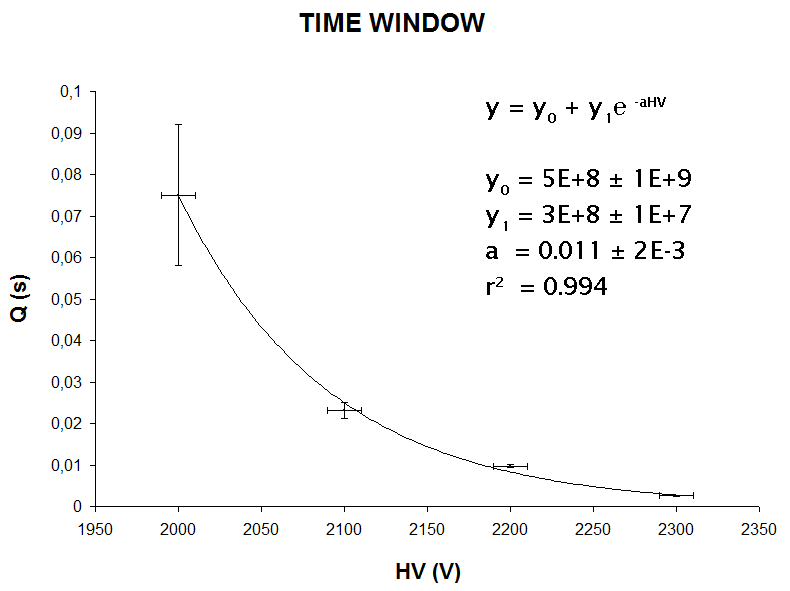
\includegraphics[width=\textwidth]{img/timeWindow.png}\ec
				\caption[Time window fit.]{Fit of the data points to an exponentially decreasing curve, whose fit parameters are shown with their error. The data is also represented with their error bars.}\label{fig:timeWin}
			\efi\vspace*{-1ex}

As discussed in Chapter \ref{chap:exp}, when the number of counts is large, ie, when the voltage is high, you should get a horizontal asymptote, whose value would be equivalent to the value of $Q$ at high number of counts. That is, when the approximation that $Q$ is of the order of the time window $\Delta T$ can be made.

The value is $\Delta T$ = 50 $\pm$ 1 ns, which agrees with $\Delta T \ll 0.15 s$. If our measuring system was very bad, a window of about $\mu$s would still be enough.
	
\subsection{Estimation of spurious coincidences and determination of the plateau}

To determine the plateau, two sets of measurements are made, as explained in Chapter \ref{chap:exp}. One by varying the voltage supplied to the detectors and the other by varying their threshold voltage. The starting voltages in each case are:

		\noindent\begin{minipage}{0.5\textwidth} 
			\bc
				Measurements varying the voltage:\\
				V$_{threshold1}$ = $-$34 $\pm$ 1 mV.\\
				V$_{threshold2}$ = $-$37 $\pm$ 1 mV.
			\ec
		\end{minipage}
		\begin{minipage}{0.5\textwidth} 
			\bc
				Measurements varying the threshold:\\
				V$_1$ = 2200 $\pm$ 1 V.\\
				V$_2$ = 2200 $\pm$ 1 V.
			\ec
		\end{minipage}

It's better to plot the curve while measuring, so that it is possible to detect and correct problems on the spot, and act accordingly.

If we plot the data of these two tables, there are some differences. The first difference is that the number of coincidences is bigger in Fig.~\ref{fig:voltage} than in Fig.~\ref{fig:threshold}, and it extends over a wider range (0-9 counts/s approximately, compared to the range of ~ 2-7 counts/s). This is consistent with the average count rate of N~/~t = 6 counts/s calculated in Chapter \ref{chap:exp}.

The contribution of random coincidences is negligible, so they are considered to neither contribute nor affect the measurements. Looking at Tables \ref{tab:voltage} and \ref{tab:threshold}, the ratio between the values of N$_{12}$  and N$_\text{random}$  is $\sim$~0.002\%.

Since we are working with the minimum threshold in the first case and the maximum voltage in the latter, the contribution of noise in the number of counts of each detector, and the spurious contributions to the number of coincidence counts should be the maximum. If these contributions are negligible, the time window has been set correctly.\vspace*{-1.5ex}

	\ctable [
	cap	    = {Determination of the plateau as a function of voltage.},
 	caption = {DETERMINATION OF PLATEAU AS A FUNCTION OF VOLTAGE. Measured voltage (HV), number of counts of detector 1 (N$_1$ / t) and detector 2 (N$_2$ / t) and coincidences (N$_{12}$ / t). From these data, the number of random coincidences N$_\text{random}$ has been calculated according to equation \ref{eq:random}. Errors and decimals presentsed are calculated as shown in Appendix \ref{chap:app3}.},
 	label   = {tab:voltage},
 	pos	    = H,
	botcap
	]
	{c c c c c}
	{}
 	{\FL
		\textbf{HV (V)} &
		\textbf{\pbox{.2\textwidth}{\pcen N$_1$ / t\\(counts/s)\\[1ex]}} &
		\textbf{\pbox{.2\textwidth}{\pcen N$_2$ / t\\(counts/s)\\[1ex]}} &
		\textbf{\pbox{.2\textwidth}{\pcen N$_{12}$ / t\\(counts/s)\\[1ex] 	}} &
		\textbf{\pbox{.2\textwidth}{\pcen N$_\text{random}$ / t\\(counts/s)\\[1ex]}} \\
		1600 $\pm$  1 & 103.7 $\pm$ 0.6 & 0.50  $\pm$ 0.04 & 0.18 $\pm$ 0.02 & 5.2E$-$6  $\pm$ 8E$-$7 \\
		1700 $\pm$  1 &  96.3 $\pm$ 0.6 & 3.0   $\pm$ 0.1  & 1.09 $\pm$ 0.06 & 2.9E$-$5  $\pm$ 2E$-$6 \\
		1800 $\pm$  1 &  92.0 $\pm$ 0.6 & 12.3  $\pm$ 0.2  & 2.8  $\pm$ 0.1  & 1.13E$-$4 $\pm$ 4E$-$6 \\
		1903 $\pm$  1 & 138.0 $\pm$ 0.7 & 249.3 $\pm$ 0.9  & 4.6  $\pm$ 0.1  & 3.4E$-$3  $\pm$ 1E$-$4 \\
		2000 $\pm$ 10 & 126.3 $\pm$ 0.6 & 143.7 $\pm$ 0.7  & 4.1  $\pm$ 0.1  & 1.81E$-$3 $\pm$ 5E$-$5 \\
		2100 $\pm$ 10 & 117.3 $\pm$ 0.6 & 347   $\pm$   1  & 4.8  $\pm$ 0.1  & 0.0041   $\pm$ 1E$-$4 \\
		2200 $\pm$ 10 & 110.0 $\pm$ 0.6 & 501   $\pm$   1  & 5.7  $\pm$ 0.1  & 0.0055   $\pm$ 1E$-$4 \\
		2300 $\pm$ 10 & 101.7 $\pm$ 0.6 & 1535  $\pm$   2  & 8.8  $\pm$ 0.2  & 0.0156   $\pm$ 1E$-$4
	\LL}\vspace*{-1.5ex}

	\ctable [
	cap	    = {Determination of the plateau as a function of the threshold.},
 	caption = {DETERMINATION OF PLATEAU AS A FUNCTION OF THRESHOLD. Measured threshold (V$_\text{threshold}$), number of counts of detector 1 (N$_1$ / t) and detector 2 (N$_2$ / t) and coincidences (N$_{12}$ / t). From these data, the number of random coincidences N$_\text{random}$ has been calculated according to equation \ref{eq:random}. Errors and decimals presented are calculated as shown in Appendix \ref{chap:app3}.},
 	label   = {tab:threshold},
 	pos	    = H,
	botcap
	]
	{c c c c c}
	{}
 	{\FL
		\textbf{\pbox{.2\textwidth}{\pcen V$_\text{threshold}$\\(mV)\\[1ex]}} &
		\textbf{\pbox{.2\textwidth}{\pcen N$_1$ / t\\(counts/s)\\[1ex]}} &
		\textbf{\pbox{.2\textwidth}{\pcen N$_2$ / t\\(counts/s)\\[1ex]}} &
		\textbf{\pbox{.2\textwidth}{\pcen N$_{12}$ / t\\(counts/s)\\[1ex]}} &
		\textbf{\pbox{.2\textwidth}{\pcen N$_\text{random}$ / t\\(counts/s)\\[1ex]}} \\
		$-$399   $\pm$ 1  & 14.7  $\pm$ 0.2 & 43.3 $\pm$ 0.4 & 2.8 $\pm$ 0.1 & 6.4E$-$5  $\pm$ 2E$-$6 \\ 
		$-$353   $\pm$ 1  & 17.7  $\pm$ 0.2 & 41.3 $\pm$ 0.4 & 2.9 $\pm$ 0.1 & 7.3E$-$5  $\pm$ 3E$-$6 \\
		$-$307   $\pm$ 1  & 21.3  $\pm$ 0.3 & 40.3 $\pm$ 0.4 & 2.8 $\pm$ 0.1 & 8.6E$-$5  $\pm$ 3E$-$6 \\ 
		$-$267   $\pm$ 1  & 25.3  $\pm$ 0.3 & 40.3 $\pm$ 0.4 & 2.7 $\pm$ 0.1 & 1.02E$-$4 $\pm$ 4E$-$6 \\
		$-$215   $\pm$ 1  & 33.3  $\pm$ 0.3 & 41.7 $\pm$ 0.4 & 3.0 $\pm$ 0.1 & 1.39E$-$4 $\pm$ 5E$-$6 \\
		$-$164   $\pm$ 1  & 51.0  $\pm$ 0.4 & 41.7 $\pm$ 0.4 & 3.0 $\pm$ 0.1 & 2.13E$-$4 $\pm$ 7E$-$6 \\
		$-$115   $\pm$ 1  & 247.0 $\pm$ 0.9 & 42.0 $\pm$ 0.4 & 3.6 $\pm$ 0.1 & 1.04E$-$3 $\pm$ 3E$-$5 \\
		$-$70.1 $\pm$ 0.1 & 1252  $\pm$ 2   & 41.3 $\pm$ 0.4 & 4.9 $\pm$ 0.1 & 0.0052   $\pm$ 1E$-$4 \\
		$-$35.2 $\pm$ 0.1 & 2492  $\pm$ 3   & 40.7 $\pm$ 0.4 & 6.3 $\pm$ 0.1 & 0.0101   $\pm$ 3E$-$4
	\LL}

			\bfi[H]
				\bc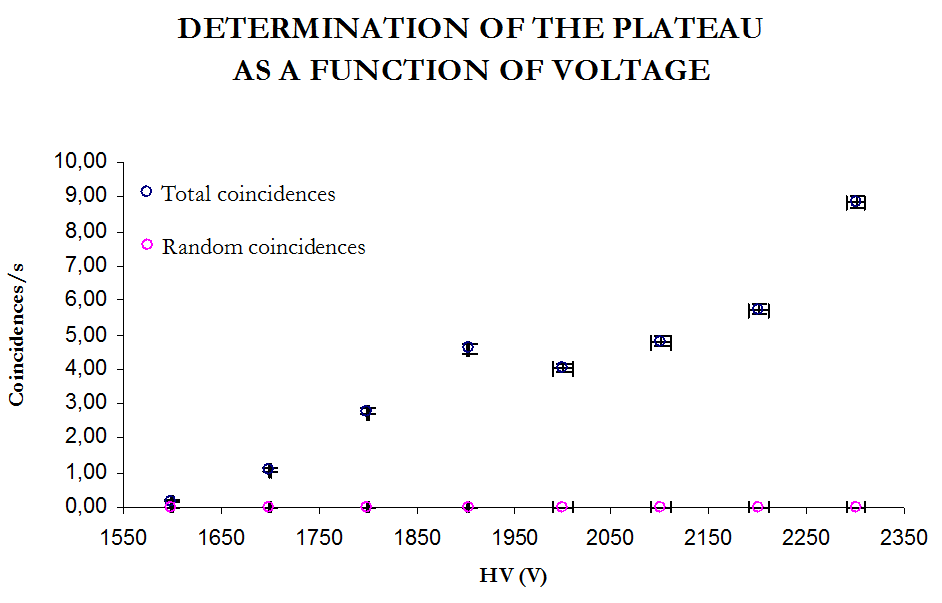
\includegraphics[width=\textwidth]{img/plateau1.png}\ec
				\caption[Coincidences against voltage.]{Coincidences against voltage.}\label{fig:voltage}
			\efi

			\bfi[H]
				\bc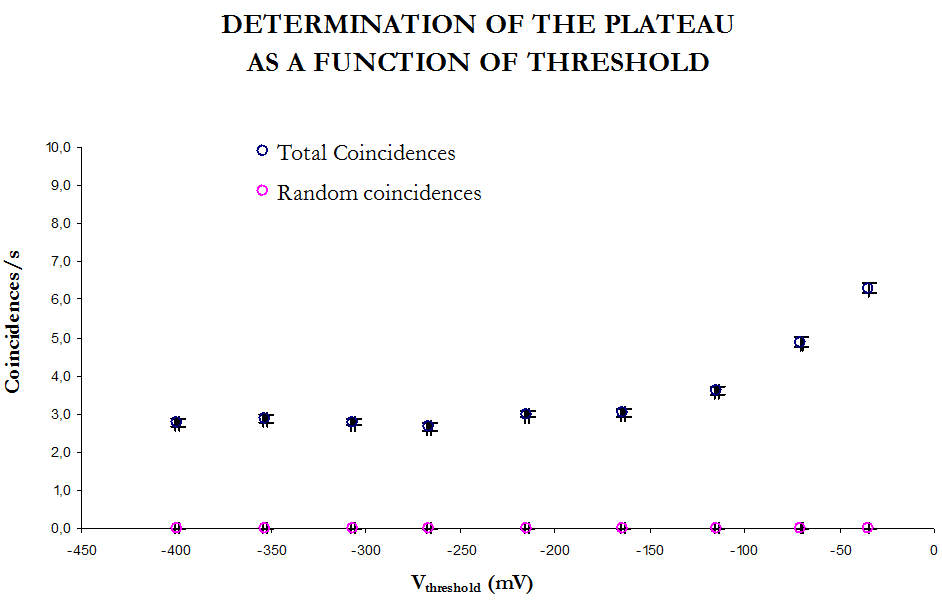
\includegraphics[width=\textwidth]{img/plateau2.png}\ec
				\caption[Coincidences against threshold.]{Coincidences against threshold.}\label{fig:threshold}
			\efi

Both the optimal working voltage and threshold for these detectors are roughly estimated from the data. They are taken from the most central part of the plateau, to avoid the areas of instability. The values are around:

	\graybox{.4}{.35}{\bc
		\noindent HV = 1900 $\pm$ 1 V \\
		\noindent V$_\text{threshold}$ = $-$200 $\pm$ 1 mV
	\ec}


The operating voltage set by the manufacturer for these scintilators can be around 2200 V, but the sensors age with use, which lowers the value of the working voltage over the years.



\section{Statistical characterization of cosmic radiation}

We can use different criteria to give the measure error $\epsilon$ in terms of percentages of the true value being in the range [$\mu - \epsilon$, $\mu + \epsilon$]. For example, according to the Gaussian distribution that represents the results, a new measure would likely fall in the range [$\mu - \sigma$, $\mu + \sigma$] with a probability of 0.683 (Appendix \ref{sec:gauss}). For this reason, $\sigma$ is also called the \textit{error of a single measurement}.


	\bi
		\item In the measurements taken at intervals of 5s, if you have a single measurement of $n$ counts, the best estimate of the true mean is this number $n$, and hence its standard deviation is $\sqrt n$ following the Poisson distribution. The data is given in the form: $n \pm \sqrt n$.

		\item From the results of the measurements every coincidences, we want to estimate their value and error under the hypothesis that, by grouping them in sets of increasing time, the values of these measures are distributed according to a  Gaussian distribution of mean $\mu$ and variance $\sigma^2$. Then we can determine that the best estimate of the mean of the distribution is the mean of the sample, $\bar{x}$. If several measurements are taken, the data is also given in the form: $\mu \pm \sqrt \mu$, with $\mu$ being the mean value.
	\ei

The values of the working voltages and thresholds for both detectors are set to the values obtained in the previous section. An example of the frequencies of the counts obtained at intervals of 5, 10 and 20s for 1 hour are shown below:

Fig.~\ref{fig:comparison} shows how as the collection time increases, the distribution is becoming increasingly flatter and wider and the maximum is shifting to the right.

Now it is time to calculate for each case the Poisson and Gaussian distributions. To compare with experimental data, we must first normalize them by dividing by the number of events $N$ that corresponds in each case.\vfill

	\ctable [
	cap	    = {Comparison of the number of coincidences.},
 	caption = {Comparison of the frequency of the number of coincidences for the measurements at intervals of 5, 10 and 20s.},
 	label   = {tab:comparison},
 	pos	    = H,
	botcap
	]
	{c c c c}
	{}
 	{\FL
		\textbf{Bin} &
		\textbf{5s} &
		\textbf{10s} &
		\textbf{20s}\\
		0 & 125 & 3  & 0 \\
		1 & 230 & 46 & 1 \\
		2 & 221 & 77 & 6 \\
		3 & 119 & 78 & 7 \\
		4 & 52  & 71 & 20 \\
		5 & 22  & 59 & 22 \\
		6 & 5   & 24 & 31 \\
		7 & 2   & 18 & 22 \\
		8 & 1   & 4  & 24 \\
		9 &     & 6  & 24 \\
		10 &    & 3  & 18 \\
		11 &    &    & 5 \\
		12 &    &    & 9 \\
		13 &    &    & 3 \\
		14 &    &    & 0 \\
		15 &    &    & 3
	\ML
		\textbf{AVERAGE}      & 1.8 & 3.6 & 7.2 \\
		\textbf{Standar Dev.} & 1.4 & 1.9 & 2.8 \\
		\textbf{N}            & 777 & 389 & 195
	\LL}\vspace*{-1ex}

	\bfi[H]
		\bc
			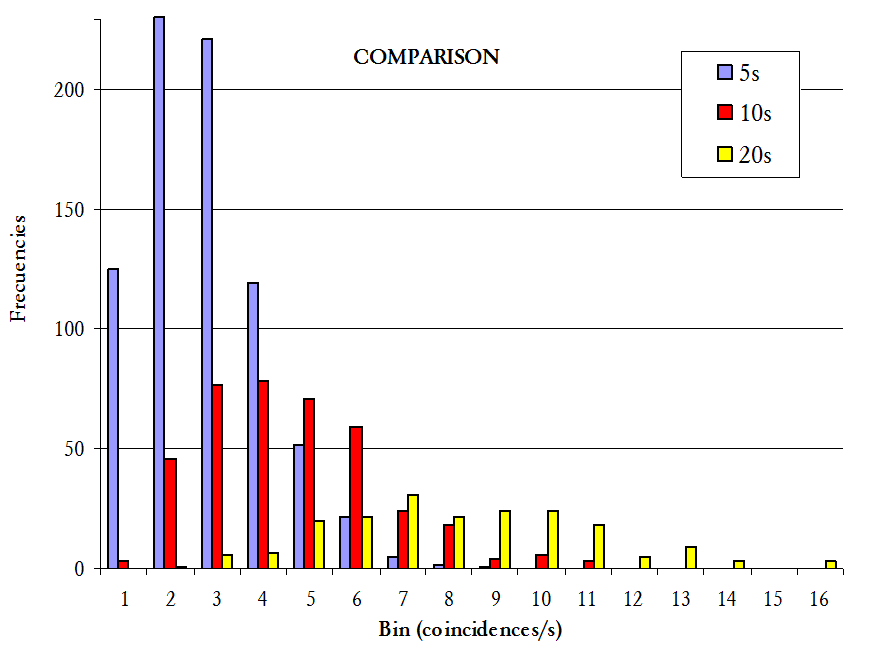
\includegraphics[width=.65\textwidth]{img/comparison.png}
			\caption
				[Frequency diagram.]
				{Frequency diagram for the number of coincidences every 5, 10, and 20s.}\label{fig:comparison}
		\ec
	\efi

\subsection{Measurements every 5s}

The table below shows that the Poisson expected values fit quite well to the experimental data within the error. However the expected values according to Gauss are a bit far from the experimental values, as expected.

	\ctable [
	cap	    = {Measurements every 5s.},
 	caption = {Measurements every 5s: Frequency of the number of coincidences and their expected value calculated using the Poisson and Gauss distributions.},
 	label   = {tab:5s},
 	pos	    = H,
	botcap
	]
	{c c c c}
	{}
 	{\FL
		\textbf{Bin} &
		\textbf{Exp.} &
		\textbf{Poisson} &
		\textbf{Gauss}\\
		0 & 0.16088 & 0.16521 & 0.12085 \\
		1 & 0.29601 & 0.29747 & 0.24884 \\
		2 & 0.28443 & 0.26780 & 0.29404 \\
		3 & 0.15315 & 0.16073 & 0.19939 \\
		4 & 0.06692 & 0.07235 & 0.07758 \\
		5 & 0.02831 & 0.02605 & 0.01732 \\
		6 & 0.00644 & 0.00782 & 0.00222 \\
		7 & 0.00257 & 0.00201 & 0.00016 \\
		8 & 0.00129 & 0.00045 & 0.00001
	\LL} 

	\bfi[H]
		\bc
			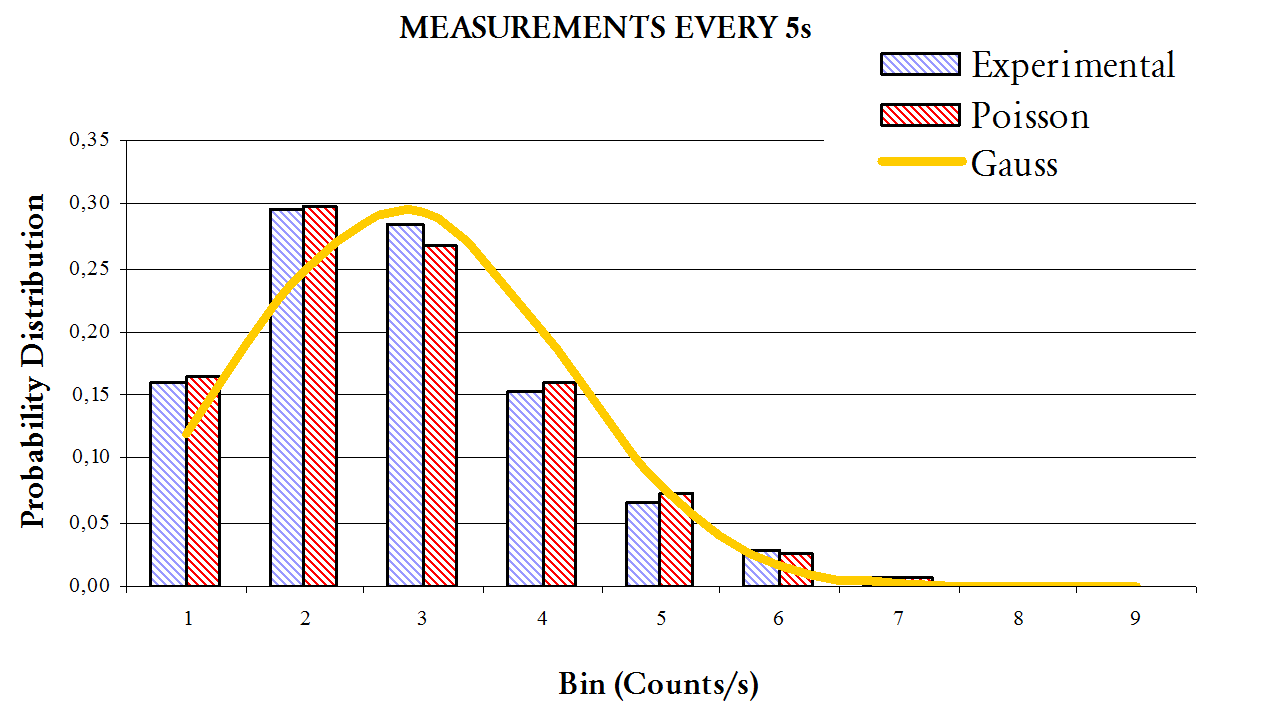
\includegraphics[width=.9\textwidth]{img/pdist1.png}
			\caption
				[Histogram for the measurements every 5s.]
				{Histogram of the number of coincidences each 5s compared to the expected value calculated using the Poisson and Gaussian distributions.}\label{fig:5s}
		\ec
	\efi

We have here a clear Poissonian curve with its maximum near the origin, as corresponds to the first part of the curve, which has a behavior proportional to $\mu^x$, while the right part of the maximum shows the typical Poisson decay, heavily dependent on the exponential decay of the $e^\mu$ distribution (Fig.~\ref{fig:5s}). 

This is corroborated by the theoretical values of the Poisson distribution, which fit very well to the data, as opposite to the Gauss distribution. The Poisson distribution is discrete so it is represented with bars, while the Gaussian is continuous so it represented with a line.

\subsection{Measurements every 10s}

If we take measurements every 10s, the data starts looking more like a Gauss distribution, although there is still no significant agreement. However, we see that the Poisson values have departed slightly from the experimental data compared with the previous table, and approaches the values as Gauss faster than experimental. This is best seen in the graphic.



We start to move away from the previous behavior, the Poissonian has shifted slightly to the right and has been flattened, seeking the Gaussian trend. Meanwhile the experimental data begins to look more like the Gaussian distribution.

	\ctable [
	cap	    = {Measurements every 10s.},
 	caption = {Measurements every 10s: Frequency of the number of coincidences and their expected value calculated using the Poisson and Gauss distributions.},
 	label   = {tab:10s},
 	pos	    = H,
	botcap
	]
	{c c c c}
	{}
 	{\FL
		\textbf{Bin} &
		\textbf{Exp.} &
		\textbf{Poisson} &
		\textbf{Gauss}\\
		0  & 0.0077 & 0.0274 & 0.0348 \\
		1  & 0.1183 & 0.0986 & 0.0824 \\
		2  & 0.1979 & 0.1773 & 0.1476 \\
		3  & 0.2005 & 0.2126 & 0.2002 \\
		4  & 0.1825 & 0.1911 & 0.2057 \\
		5  & 0.1517 & 0.1375 & 0.1600 \\
		6  & 0.0617 & 0.0824 & 0.0942 \\
		7  & 0.0463 & 0.0423 & 0.0420 \\
		8  & 0.0103 & 0.0190 & 0.0142 \\
		9  & 0.0154 & 0.0076 & 0.0036 \\
		10 & 0.0077 & 0.0027 & 0.0007
	\LL}


	\bfi[H]
		\bc
			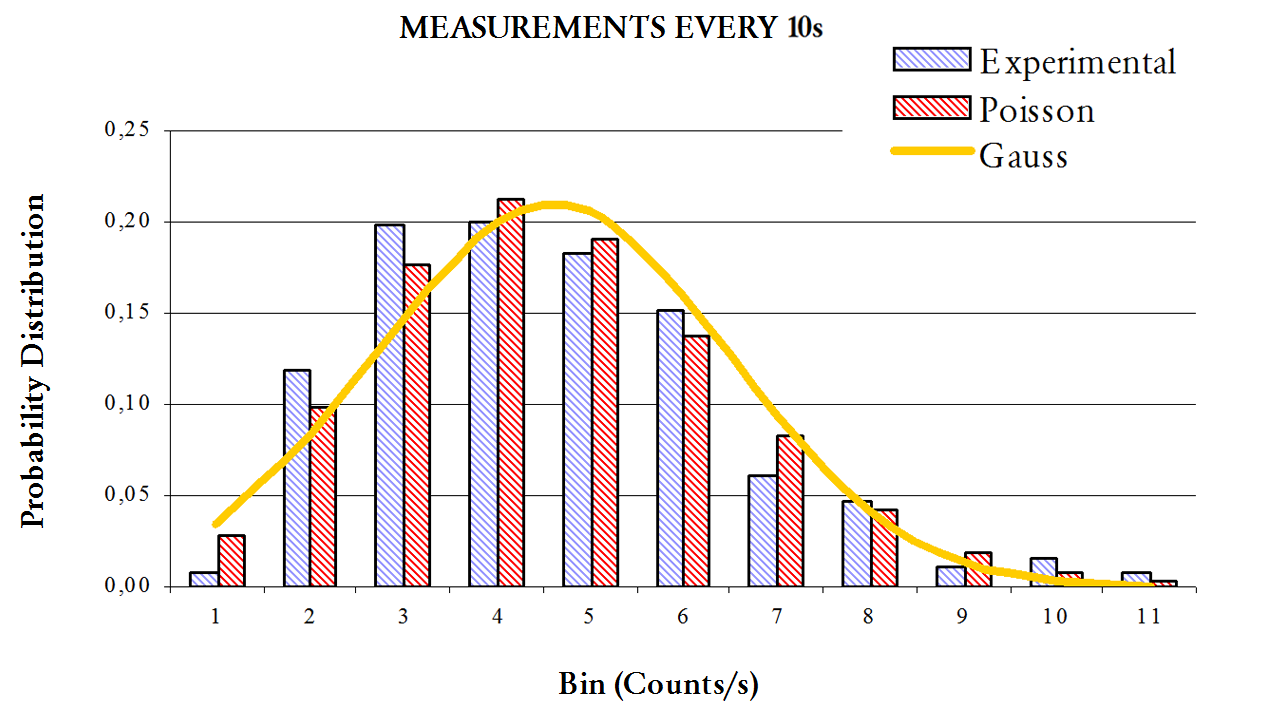
\includegraphics[width=.9\textwidth]{img/pdist2.png}
			\caption
				[Histogram for the measurements every 10s.]
				{Histogram of the number of coincidences grouped in intervals of 10s compared to the expected value calculated using the Poisson and Gaussian distributions.}\label{fig:10s}
		\ec
	\efi

\subsection{Measurements every 20s}

In this case, the Gauss distribution is even more similar to the experimental data, while Poisson continues to move away from their initial values. This will become evident in the graph below.

The data is nearly Gaussian, the Poissonian has abandoned its asymmetrical shape to become increasingly symmetrical, the peak has shifted to the right in search of the Gaussian and has flattened a little. With the increase of the measurement interval, the Poisson distributions gets closer to a Gaussian shape.

The experimental data also agree quite well with the Gaussian, removing some fluctuations like the maximum in bin 7 which is nothing more than a reminder of their old Poissonian tendency.

The shift of the Poisson distribution into a Gaussian is quite fast: with a difference of 5 or 10s in the measurement range, a fairly sharp change is seen in the shape of the distribution. This is remarkable because this distribution is modulated by only one parameter. The average $\mu$ alone makes the curve to flatter, moves its maximum and changes its width.

	\ctable [
	cap	    = {Measurements every 20s.},
 	caption = {Measurements every 20s: Frequency of the number of coincidences and their expected value calculated using the Poisson and Gauss distributions.},
 	label   = {tab:20s},
 	pos	    = H,
	botcap
	]
	{c c c c}
	{}
 	{\FL
		\textbf{Bin} &
		\textbf{Exp.} &
		\textbf{Poisson} &
		\textbf{Gauss}\\
		0  & 0     & 0.001 & 0.004 \\
		1  & 0.005 & 0.005 & 0.010 \\
		2  & 0.031 & 0.020 & 0.023 \\
		3  & 0.036 & 0.047 & 0.044 \\
		4  & 0.103 & 0.085 & 0.074 \\
		5  & 0.113 & 0.121 & 0.107 \\
		6  & 0.159 & 0.145 & 0.135 \\
		7  & 0.113 & 0.149 & 0.149 \\
		8  & 0.123 & 0.133 & 0.142 \\
		9  & 0.123 & 0.106 & 0.118 \\
		10 & 0.092 & 0.076 & 0.085 \\
		11 & 0.026 & 0.050 & 0.054 \\
		12 & 0.046 & 0.030 & 0.029 \\
		13 & 0.015 & 0.016 & 0.014 \\
		14 & 0     & 0.008 & 0.006 \\
		15 & 0.015 & 0.004 & 0.002
	\LL} 

	\bfi[H]
		\bc
			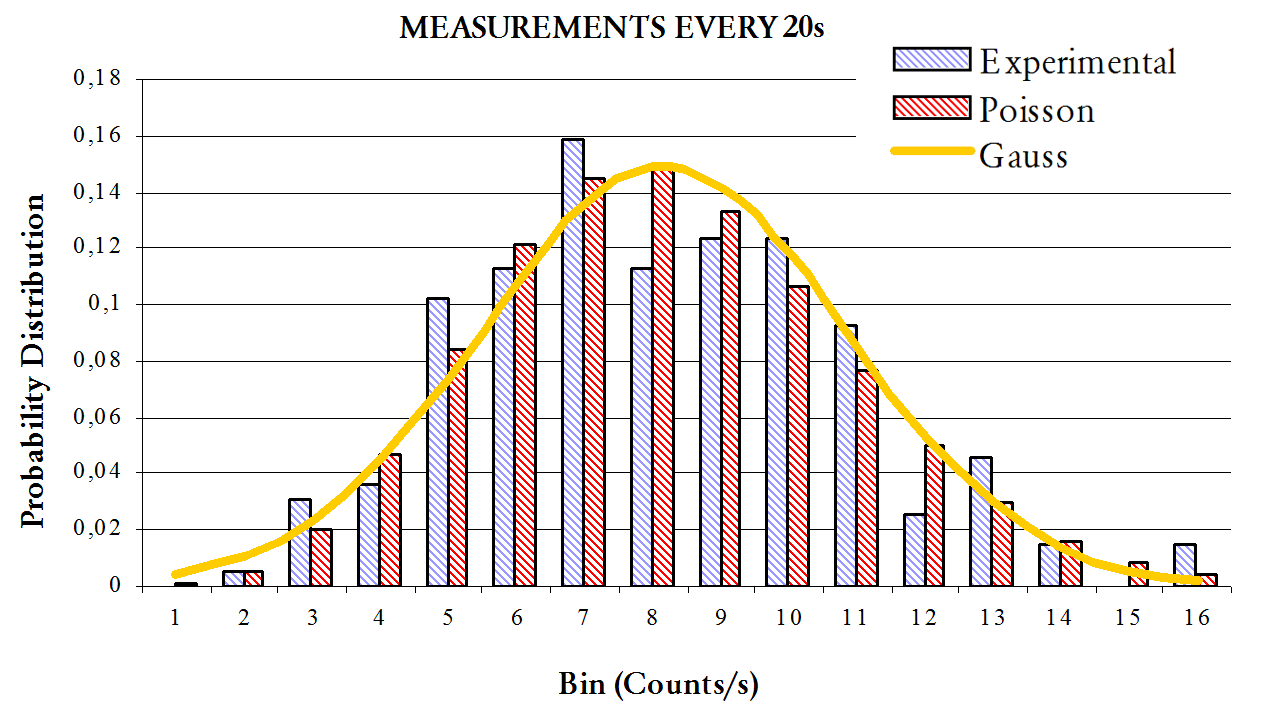
\includegraphics[width=.9\textwidth]{img/pdist3.png}
			\caption
				[Histogram for the measurements every 20s.]
				{Histogram of the number of coincidences grouped in intervals of 20s together with the expected values (solid lines) calculated according to the Poisson and Gauss distributions.}\label{fig:20s}
		\ec
	\efi

\subsection{Chi-square test results}

Given that the possible values of $\chi^2$ are distributed according to the Chi-squared distribution, whose expected value is equal to the number of degrees of freedom $\nu$, which in turn is equal to the number of experimental points $n$ (which is the number of corresponding frequencies in each case), minus the number of parameters or constraints $k$, which in this case is found to be 2, the mean $\mu$ and the number of data $N$, and whose standard deviation is $\sigma = \sqrt{2\nu}$
(Appendix \ref{sec:chi2}) it is possible to establish a measure of the quality of fit (Table \ref{tab:chieval}):


	\ben
		\item If the fit provides a $\chi^2$ that is less than 3$\sigma$ of its expected value, we can speak of an acceptable fit.

		\item If the $\chi^2$ value is much less of its expected value, presumably the assigned errors $\sigma_i$ have been overestimated. In this case, the experiment must be repeated.

		\item If the $\chi^2$ is at more than 3$\sigma$ from its expected value, several problems may be the cause:
			\bi 
				\item The set of measurements is incorrect.
				\item The assigned errors are too small.
				\item The model function is inadequate.
			\ei
	\een

As a general rule, it is assumed that being $\chi_\text{exp}^2$ the value found for $\chi^2$, if

	\bc $P \left(\chi^2 < \chi_\text{exp}^2\right) = \sum_{-\infty}^{\chi_c^2} P_\nu(x) \,dx$\ec

is between 0.1 and 0.9, the hypothesis is correct, given that this judgment has a confidence level equal to CL = $P \left(\chi^2 < \chi_\text{exp}^2\right) \times$ 100\% (Appendix \ref{sec:chi2}).

For a total of 8 frequencies in the first case (5s), 10 frequencies in the second (10s) and 15 in the third (20s), and having two constraints in all cases, since the Gaussian limit of the Poisson distribution still has one parameter (the mean $\mu$), values of 6, 8 and 13 are obtained respectively for $\nu$. The confidence intervals between which $\chi^2 = \chi_\text{exp}^2$ is situated can be calculated for the different degrees of freedom according to Table \ref{tab:chieval}:

	\ctable [
	cap	    = {Intervals between which $\chi_c^2$ is located.},
 	caption = {Intervals between which $\chi_c^2$ is located according to the different degrees of freedom obtained in this section. P values are taken from Table \ref{tab:chieval}.},
 	label   = {tab:intervals},
 	pos	    = H,
	botcap
	]
	{c c c c c}
	{}
 	{\FL
		\textbf{$\chi_c^2$} &
		\textbf{$\nu$ = 6}  &
		\textbf{$\nu$ = 8}  &
		\textbf{$\nu$ = 13} &
		\textbf{$P \left(\chi^2 < \chi_\text{exp}^2\right)$}\\[1ex]
		$\nu \pm 3\sigma$ & ($-$4.390 $< \chi_c^2 <$ 16.392) & ($-$4 $< \chi_c^2 <$ 20) & ($-$2.297 $< \chi_c^2 <$ 28.297) & 0.99\\[1.5ex]
		$\nu \pm 2\sigma$ & ($-$0.900 $< \chi_c^2 <$ 12.928) & (0 $< \chi_c^2 <$ 16)  & (2.802 $< \chi_c^2 <$ 23.198)  & 0.96\\[1.5ex]
		$\nu \pm \sigma$  & (2.536 $< \chi_c^2 <$ 9.464)   & (4 $< \chi_c^2 <$ 12)  & (7.901 $< \chi_c^2 <$ 18.099)  & 0.85\\[1.5ex]
		$\nu$             & $\chi_c^2$ = 6                 & $\chi_c^2$  = 8        & $\chi_c^2$  = 13               & 0.55
	\LL} 

Since this table is very limited because it shows the value of $P$ for a whole interval, the exact value of the confidence level corresponding to each given value of $\chi_c^2$ obtained experimentally using the program at the end of Appendix \ref{chap:app4}. The $\chi_c^2$ obtained from the data in Tables \ref{tab:5s}-\ref{tab:20s} are shown below:

	\ctable [
	cap	    = {Values of time, degrees of freedom and $\chi^2$.},
 	caption = {Values of time, degrees of freedom and $\chi^2$ obtained for the Poisson distribution or P (x) and Gauss or G (x) with their confidence level calculated according the \code{cl.cpp} program.},
 	label   = {tab:clcpp},
 	pos	    = H,
	botcap
	]
	{c c c c c c}
	{}
 	{\FL
		\textbf{Time (s)} &
		\textbf{$\nu$}  &
		\textbf{\pbox{.1\textwidth}{\pcen$\chi_\text{exp}^2$ P(x)\\[1ex]}}  &
		\textbf{\pbox{.2\textwidth}{\pcen Confidence level according to \code{cl.cpp}\\[1ex]}} &
		\textbf{\pbox{.1\textwidth}{\pcen$\chi_\text{exp}^2$ G(x)}}  &
		\textbf{\pbox{.2\textwidth}{\pcen Confidence level according to \code{cl.cpp}\\[1ex]}} \\
		5  & 6  & 0.004 & 0.998002 & 0.323 & 0.850866 \\
		10 & 8  & 0.050 & 0.97531  & 0.178 & 0.914846 \\
		20 & 13 & 0.092 & 0.955042 & 0.153 & 0.926353
	\LL} 

With these values of $\chi^2$ and our number of constraints (2) we run the program \code{cl.cpp} (Appendix \ref{sec:chi2}) and obtain the confidence levels shown for each of the values of $\chi^2$.

There is certain compatibility observed between the values of \code{cl.cpp} and Table \ref{tab:intervals}, as in the case of $\nu$ = 6 for example, both the value of $\chi_\text{exp}^2 P(x)$ and $\chi_\text{exp}^2 G(x)$ are less than 3$\sigma$ of its expected value $\nu$, since they are in the range $\nu \pm 2\sigma$, so according to item 1 of this section, both fits would be good, but in the case of $P(x)$ the program gives a higher confidence value than for $G(x)$.

The value of $\chi^2$ grows for the Poisson distribution as we increase the measuring time, so the confidence level decreases from 99.8\% to 95.5\%. According to this, we would say with certainty that the experimental data fit a Poisson distribution in the measurements every 5s, with a confidence of 99.8\%.

Furthermore, the effect of grouping measurements in greater time intervals, makes the $\chi^2$ of the Gaussian distribution to decrease, so its confidence level increases from 85.1\% to 92.6\%, although without reaching the values of the Poissonian. Therefore, in the case of measurements of 20s, we could say that the data follows a Gaussian with a security of \enquote{only} the 92.6\%, which is not bad although our confidence is lower than in the case of Poisson at 5s.

It follows that, in the first case, we must reject the hypothesis of the Gaussian, in the second case is still Poissonian, and in the third case there is no reason to rule out the Gaussian assumption, as the confidence level, although lower, is high enough.


If coincidences were grouped into larger time intervals, of 40s or minutes, we would get increasingly higher values of $\chi^2$ for the Poisson distribution and lower for the Gaussian distribution, which would translate into a higher level of confidence for Gauss, confirming the hypothesis that \textbf{cosmic radiation has a Gaussian probability distribution}. In fact, some books \cite{kno:79} say that when the mean of a distribution (binomial at least) is greater than 30 events, the distribution is Gaussian.

And so the statistical nature of cosmic radiation is well demonstrated.



\section{Separation of the hard component of coincidences}


In this section it is important to wait longer (around an hour) for each measurement, in order to get a number of counts with an error of $\sim$5--10\%. The distance between scintillators is 30.0 $\pm$ 0.1 cm. The method of analysis discussed in section \ref{chap:exp} is broken down here briefly.

The fits obtained for Al and Pb must give compatible values for the value of the components at zero thickness. Typical experimental values for the attenuation in lead and aluminium are (errors and decimals presented are calculated according to Appendix~\ref{chap:app3}):

	\ctable [
	cap	    = {Attenuation in lead.},
 	caption = {Increasing thickness of the layers of Pb (an error of $\pm$ 1 mm has been considered) along with the number of coincidences ($N_{12}$ / t). Measurements with the lead blocks were also made, as well as mixing blocks and thin layers.},
 	label   = {tab:lead},
 	pos	    = H,
	botcap
	]
	{c c c}
	{}
 	{\FL
		\textbf{x (cm)} &
		\textbf{\pbox{.3\textwidth}{\pcen$N_{12}$ / t\\(coinc./s)\\[1ex]}}  &
		\textbf{\pbox{.3\textwidth}{\pcen Error / t\\(coinc./s)\\[1ex]}}  \\
		0    & 0.82 & 0.03 \\
		0.3  & 0.88 & 0.04 \\
		0.6  & 0.86 & 0.04 \\
		0.9  & 0.78 & 0.04 \\
		1.2  & 0.71 & 0.03 \\
		 5   & 0.62 & 0.03 \\
		10   & 0.63 & 0.03 \\
		15   & 0.56 & 0.03 \\
		20   & 0.53 & 0.03 \\
		20.9 & 0.55 & 0.03 \\
		21.2 & 0.55 & 0.03 \\
		21.5 & 0.55 & 0.03 \\
		25   & 0.51 & 0.03
	\LL}

	\ctable [
	cap	    = {Attenuation in aluminium.},
 	caption = {Increasing thickness of the layers of Al (an error of $\pm$ 1 mm has been considered) along with the number of coincidences ($N_{12}$ / t).},
 	label   = {tab:alum},
 	pos	    = H,
	botcap
	]
	{c c c}
	{}
 	{\FL
		\textbf{x (cm)} &
		\textbf{\pbox{.3\textwidth}{\pcen$N_{12}$ / t\\(coinc./s)\\[1ex]}}  &
		\textbf{\pbox{.3\textwidth}{\pcen Error / t\\(coinc./s)\\[1ex]}}  \\
		0  & 1.00 & 0.04 \\
		3  & 0.90 & 0.04 \\
		6  & 0.91 & 0.04 \\
		9  & 0.85 & 0.04 \\
		12 & 0.81 & 0.04 \\
		15 & 0.73 & 0.03 \\
		18 & 0.78 & 0.04 \\
		21 & 0.74 & 0.04 \\
		24 & 0.73 & 0.03 \\
		27 & 0.78 & 0.04
	\LL}


	\graybox{.9}{.75}{
		\bc\textcolor{gray}{\Large{\sffamily Exponential Fit:}}\ec

		Should conform to the function:

		\bc$f(x) = A_1e^{-\frac{x}{b_1}} + A_2e^{-\frac{x}{b_2}}$\ec

		where $b_i = \frac{\Lambda_i}{\rho_\text{Pb}}$, and the slower exponential decay corresponds to the hard component.\\

		Considering for example, the first exponential as the correspondent to the hard component, $A_1$ would be the amount of $\mu^\pm$ (the hard component) at zero thickness, and $A_2$ the amount of e$^\pm$ (the soft component) at zero thickness. The value of $f(x)$ at $x$ = 0 gives the sum of these two contributions.\\

		If the exponential part of the soft component falls much faster than the hard one, it means that $b_2$ is much smaller than $b_1$, and in the appropriate data range ($b_2 \ll x \ll b_1$) the second exponential tends to zero. Then, $f(x)$ behaves as a straight line intersecting the Y axis $A_1$:
		\bc$f(x) \sim A_1\left(1 - \frac{x}{b_1}\right) \qquad$ in $b_2 \ll x \ll b_1$\ec

		With the $b_1$ obtained from this fit, is easy to see that the experimental values of $x$ are in the proper range ($x_i \ll b_1$) and that this linear approximation is valid.
	}

\subsection{Fit for Lead}

For the \textbf{soft component} we obtain $b_1 = \mu_1^{-1} = \Lambda_1 / \rho_\text{Pb}$ = 4.7 $\pm$  0.3 cm (Fig. \ref{fig:lead}) so:\vspace{-1ex}
\bc $\mu_1$ = 0.213 $\pm$ 0.009 cm$^{-1} \qquad$ and $\qquad \Lambda_1$ = 5 $\pm$ 2 g cm$^{-2}$\ec


and taking the value of $A_1$ (the rate of soft component at zero thickness), if $S$ is the surface of the detectors, the flux of soft component is,

	\bfi[H]
		\begin{minipage}{.8\textwidth}
			\bc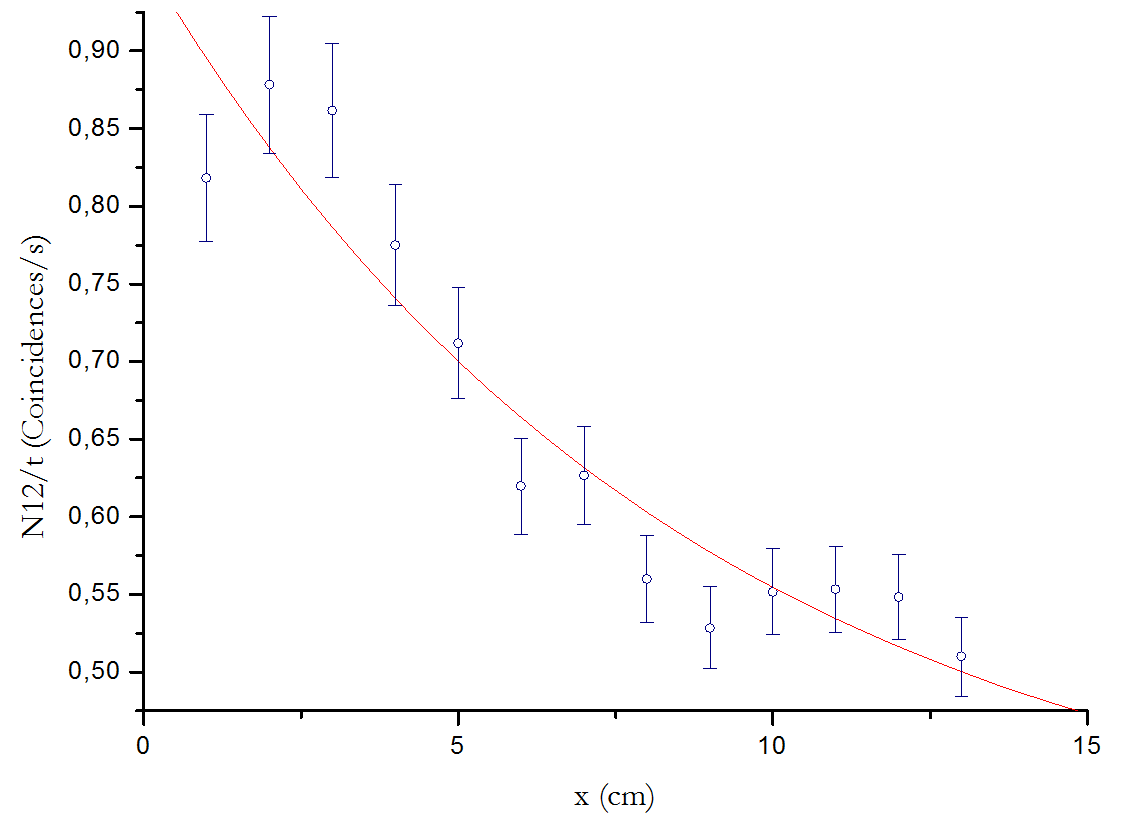
\includegraphics[width=\textwidth]{img/atenuationPb.png}\ec
		\end{minipage}\begin{minipage}{.2\textwidth}
			$\chi^2$ = 0.00248\\
			$r^2$ = 0.89735\\

			$A_1$ = 0.4 $\pm$ 0.2\\
			$b_1$ = 4.7 $\pm$ 0.3\\

			$A_2$ = 0.6 $\pm$ 0.1\\
			$b_2$ = 9 $\pm$ 5\\
		\end{minipage}
		\caption
			[Attenuation in lead.]
			{Attenuation of cosmic radiation passing through layers of lead, with error bars and fit results.}\label{fig:lead}
	\efi

\graybox{.4}{.35}{\bc $J_s = \frac{N_s/t}{S}$ = 13 $\pm$ 6 m$^{-2}$s$^{-1}$\ec}

The errors are calculated according to Appendix \ref{chap:app3}. The value of $J$ is a bit low compared to the theoretical value in Table \ref{tab:rppp}, this is due to the effect of the geometric efficiency, given that detectors have to be separated by a distance.

For the \textbf{hard component}, $b_2 = \mu_2^{-1} = \Lambda_2 / \rho_\text{Pb}$ = 9 $\pm$ 5 cm, which:

\bc $\mu_2$ = 0.11 $\pm$ 0.06 cm$^{-1} \qquad$ and $\qquad \Lambda_2$ = 102 $\pm$ 55 g cm$^{-2}$\ec

and the flux of the hard component is,

\graybox{.4}{.35}{\bc $J_h = \frac{N_h/t}{S}$ = 19 $\pm$ 3 m$^{-2}$s$^{-1}$\ec}

Its value is also far from the theoretical value shown in Table \ref{tab:rppp}, however, the linear absorption coefficient $\mu$ for muons is lower than for the soft component, as expected.

\graybox{.9}{.75}{
	As already mentioned, if the soft component falls much faster than the hard one, since $b_1$ would be much lower than $b_2$, in an appropriate data range $b_1 \ll x \ll b_2$, the first exponential tends to zero, and $f(x)$ behaves like a straight line intersecting the Y axis in $A_2$:
		\bc$f(x) \sim A_2\left(1 - \frac{x}{b_2}\right) \qquad$ in $b_1 \ll x \ll b_2$\ec
	In this part, error handling is not needed since a qualitative approach is enough, and we choose the range below and make a linear fit to it:\\

	\begin{minipage}{.3\textwidth}
		\begin{tabular}{ c c }
			\hline
  			\textbf{x (cm)} &
			\textbf{$N_{12}/t$} \\
			10 & 0.63 \\
			15 & 0.56 \\
			20 & 0.53 \\
			25 & 0.51 \\
			\hline
		\end{tabular}
	\end{minipage}\begin{minipage}{.7\textwidth}
		$y$ = 0.690 $\pm$ 0.008$x$\\
		$r^2$ = 0.923\\

		$A_2$ = 0.6898 s$^{-1}$\\
		$b_2$ = $A_2$/0.0076 = 90.76 cm$^{-1}$s$^{-1}$
	\end{minipage}\vspace*{2ex}

	With the value of $b_2$ obtained from this fit, we can check that the experimental values of $x$ are in the proper range ($x_i \ll b_2$) and that this linear approximation is valid. In this case the value of $b_2$ which is 10 times larger than the one obtained previously, but indeed in the range of $x$ chosen $x \ll b_2$ is fulfilled, so the linear approximation in that range is valid, and the value of $A_2$ (hard component at zero thickness) is compatible with the value obtained before.
}



\subsection{Fit for Aluminum}

	\bfi[H]
		\begin{minipage}{.78\textwidth}
			\bc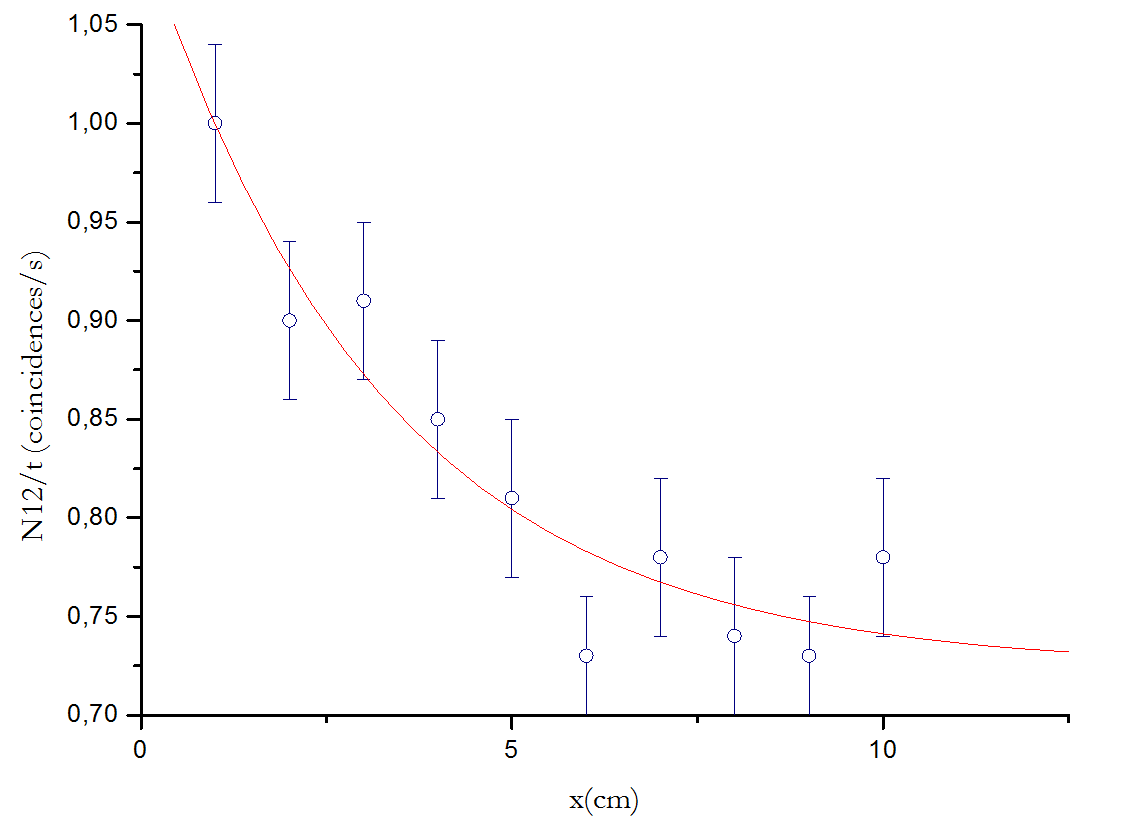
\includegraphics[width=\textwidth]{img/atenuationAl.png}\ec
		\end{minipage}\begin{minipage}{.22\textwidth}
			$\chi^2$ = 0.00124\\
			$r^2$ = 0.89909\\

			$A_1$ = 0.68 $\pm$ 0.04\\
			$b_1$ = 3.5 $\pm$ 0.4\\

			$A_2$ = 0.37 $\pm$ 0.06\\
			$b_2$ = 3 $\pm$ 1\\
		\end{minipage}
		\caption
			[Attenuation in lead.]
			{Attenuation of cosmic radiation passing through layers of aluminium, with the fit and error bars.}\label{fig:alum}
	\efi


For the \textbf{hard component}, $b_1 = \mu_1^{-1} = \Lambda_1 / \rho_\text{Al}$ = 3.5 $\pm$ 0.4 cm, so we get:

\bc $\mu_1$ = 0.29 $\pm$ 0.03 cm$^{-1} \qquad$ and $\qquad \Lambda_1$ = 9 $\pm$ 1 g cm$^{-2}$\ec

and the flux of the hard component is,

\graybox{.4}{.35}{\bc $J_h = \frac{N_h/t}{S}$ = 22 $\pm$ 1 m$^{-2}$s$^{-1}$\ec}

The errors were calculated according to Appendix \ref{chap:app3}. Again it is observed that the value remains low compared to the theoretical value in Table \ref{tab:rppp}, and for the same reason.

For the \textbf{soft component} we obtain $b_2 = \mu_2^{-1} = \Lambda_2 / \rho_\text{Pb}$ = 3 $\pm$ 1 cm so:

\bc $\mu_2$ = 0.3 $\pm$ 0.1 cm$^{-1} \qquad$ and $\qquad \Lambda_2$ = 8 $\pm$ 3 g cm$^{-2}$\ec

and the flux of soft component is,

\graybox{.4}{.35}{\bc $J_s = \frac{N_s/t}{S}$ = 12 $\pm$ 2 m$^{-2}$s$^{-1}$\ec}

Again, it is a bit low compared to the theoretical value in Table \ref{tab:rppp}, but the $\mu$ for muons is again smaller than for electrons.

The results can also be explained by the fact that the roof attenuates some part of the soft component, but not the hard one, so less soft component is measured compared to what would be obtained under different conditions.


\graybox{.9}{.75}{
	As before, if the soft component falls much faster than the hard one, since $b_2$ would be much lower than $b_1$, in an appropriate data range $b_2 \ll x \ll b_1$, the first exponential tends to zero, and $f(x)$ behaves like a straight line intersecting the Y axis in $A_1$:
		\bc$f(x) \sim A_1\left(1 - \frac{x}{b_1}\right) \qquad$ in $b_2 \ll x \ll b_1$\ec

	Linear fit to the data range on the left:\\

	\begin{minipage}{.3\textwidth}
		\begin{tabular}{ c c }
			\hline
  			\textbf{x (cm)} &
			\textbf{$N_{12}/t$} \\
			12 & 0.81 \\
			18 & 0.78 \\
			21 & 0.74 \\
			24 & 0.73 \\
			\hline
		\end{tabular}
	\end{minipage}\begin{minipage}{.7\textwidth}
		$y$ = 0.9019 $\pm$ 0.0074$x$\\
		$r^2$ = 0.9529\\

		$A_1$ = 0.9019 s$^{-1}$\\
		$b_1$ = $A_1$/0.0074 = 121.9 cm$^{-1}$s$^{-1}$
	\end{minipage}\vspace*{2ex}

	With the value of $b_1$ obtained from this fit, we can check that the experimental values of $x$ are in the proper range ($x_i \ll b_1$) and that this linear approximation is valid.\\
}
\graybox{.9}{.75}{
	In this case the value of $b_1$ which is 10 times larger than the one obtained previously, but indeed in the range of $x$ chosen $x \ll b_1$ is fulfilled, so the linear approximation in that range is valid, and the value of $A_1$ (hard component at zero thickness) is compatible with the value obtained before.
}

The number of particles of the soft and hard component obtained at zero thickness  for Al and Pb should be compatible, as shown in the table below.

	\ctable [
	cap	    = {Hard and soft components at zero thickness.},
 	caption = {Hard and soft components at zero thickness.},
 	label   = {tab:atzero},
 	pos	    = H,
	botcap
	]
	{l c c c}
	{}
 	{\FL
		&
		\textbf{Hard} &
		\textbf{Soft} &
		\textbf{Total} \\
		Lead      & 
		19 $\pm$ 3 m$^{-2}$s$^{-1}$ & 
		13 $\pm$ 6 m$^{-2}$s$^{-1}$ &
		32 $\pm$ 9 m$^{-2}$s$^{-1}$ \\
		Aluminium &
		22 $\pm$ 1 m$^{-2}$s$^{-1}$ &
		12 $\pm$ 2 m$^{-2}$s$^{-1}$ &
		34 $\pm$ 3 m$^{-2}$s$^{-1}$
	\LL}

Remember that these data have to be taken at $d$ = 30 cm. and thickness $x$ = 0 cm. In the case of the hard component, there is a bit larger difference between the two results at zero thickness, but this difference is at the limit of error, while for the soft component there is a great agreement.


\section{Calculation of the geometric efficiency}

Taking the data obtained in the previous section for the hard and soft components (with detectors at $d$ = 30.0 $\pm$ 0.1 cm), and the first experimental data we obtained in this section for $d$ = 0 cm. The following table is obtained:

	\ctable [
	cap	    = {Summary of experimental data obtained for $J$ in the previous section.},
 	caption = {Summary of experimental data obtained for $J$ in the previous section contrasted with theory and with data for $d$ = 0.},
 	label   = {tab:summary},
 	pos	    = H,
	botcap
	]
	{l c c c c}
	{}
 	{\FL
		&
		\multicolumn{2}{c}{\textbf{Hard (m$^{-2}$s$^{-1}$)}} &
		\multicolumn{2}{c}{\textbf{Soft (m$^{-2}$s$^{-1}$)}} \\
		\cmidrule(rl){2-3}\cmidrule(l){4-5}
		Theory      & 
		\multicolumn{2}{c}{130} &
		\multicolumn{2}{c}{ 50} \\
		\cmidrule(r){1-1}\cmidrule(rl){2-3}\cmidrule(l){4-5}
		\multirow{2}{.2\textwidth}{Experiment at $d$ = 30 cm and thickness $x$ = 0} &
		Lead & Aluminum & Lead & Aluminum \\ 
		& 19 $\pm$ 3 & 22 $\pm$ 1 & 13 $\pm$ 6 & 12 $\pm$ 2 \\
		& & & & \\
		\cmidrule(r){1-1}\cmidrule(l){2-5}
		\pbox{.2\textwidth}{\pcen Experiment at $d$ = 0 cm\\[1ex]} &
		\multicolumn{4}{c}{34.2 $\pm$ 0.6 (Total flux)} 
	\LL}


There is a growth in the number of total particles that are detected with the scintillators attached. In this section, one of the possible causes of the inconsistency between theory and experiment mentioned in the previous section will be addressed.

\subsection{Experimental measurements}

For each value of the distance between scintillators, six measurements of the coincidences are taken, in order to calculate the average, thus the error is given by the dispersion $\sigma$ (Appendix \ref{chap:app3}). The duration of each measurement is six minutes. The working conditions are set to these values:

\bc
HV$_1$ = 1900 V, V$_\text{threshold}$ = $-$200 mV\\
HV$_2$ = 1900 V, V$_\text{threshold}$ = $-$200 mV\ec

The data in Table \ref{tab:avcoinc} is obtained.

	\ctable [
	cap	    = {Coincidences as a function of distance.},
 	caption = {Increasing values of $d$ (an error of $\pm$ 1 mm has been considered) along with the number of averaged coincidences (N$_{12}$ av./t). It also presents the ratio N$_{12}$(d) /N$_{12}$(0) , where N$_{12}$(d) is the number of coincidences with the detectors at a distance d, and N$_{12}$(0) the number of coincidences when the detectors are together. Errors and decimals presented are calculated as shown in Appendix \ref{chap:app3}.},
 	label   = {tab:avcoinc},
 	pos	    = H,
	botcap
	]
	{c c c}
	{}
 	{\FL
		\textbf{d (cm)} &
		\textbf{\pbox{.3\textwidth}{\pcen N$_{12}$ av./t\\(counts / s)\\[1ex]}} &
		\textbf{\pbox{.3\textwidth}{\pcen N$_{12}$(d) /N$_{12}$(0) \\(counts / s)\\[1ex]}}\\
		0.0  & 1.06  $\pm$ 0.02 & 1.00   $\pm$ 0.03 \\
		5.5  & 0.46  $\pm$ 0.01 & 0.43   $\pm$ 0.02 \\
		8.5  & 0.29  $\pm$ 0.01 & 0.27   $\pm$ 0.01 \\
		11.0 & 0.21  $\pm$ 0.01 & 0.20   $\pm$ 0.01 \\
		15.5 & 0.158 $\pm$ 0.008 & 0.149 $\pm$ 0.008 \\
		19.5 & 0.100 $\pm$ 0.006 & 0.094 $\pm$ 0.006 \\
		23.5 & 0.092 $\pm$ 0.006 & 0.086 $\pm$ 0.006 \\
		25.0 & 0.069 $\pm$ 0.006 & 0.065 $\pm$ 0.005
	\LL}

In this case the ratio of N$_{12}$(d) and N$_{12}$(0) is the geometric efficiency  calculated from experimental data for each distance, as explained in chapter \ref{chap:exp}. We see that as the distance between scintillators increases, the efficiency decreases by 94\% from 1 for the most ideal case (with the scintillators at $d$ = 0), to 0.06 for a distance of 25 cm. Even when separated 5 cm we have a loss of just over 50\%.

\subsection{Monte-Carlo simulation (Appendix \ref{chap:app2})}

Simulate a flux of 10000 particles for the same distances used in the experimental measurements.  You should obtain something as the data in Table \ref{tab:geff}.

	\ctable [
	cap	    = {Geometric efficiency.},
 	caption = {Increasing values of d (with an error of $\pm$ 1 mm) with the number of counts that fell within the detector (n). The geometric efficiency is also presented. Calculation errors are not considered in these data.},
 	label   = {tab:geff},
 	pos	    = H,
	botcap
	]
	{c c c}
	{}
 	{\FL
		\textbf{d (cm)} &
		\textbf{\pbox{.3\textwidth}{\pcen n\\(counts)\\[1ex]}} &
		\textbf{\pbox{.3\textwidth}{\pcen Geom. eff \\$\epsilon$\\[1ex]}}\\
		0.0  & 10000 & 1 \\
		5.5  & 7585  & 0.7585 \\
		8.5  & 6647  & 0.6647 \\
		11.0 & 6026  & 0.6026 \\
		15.5 & 5236  & 0.5236 \\
		19.5 & 4751  & 0.4751 \\
		23.5 & 4398  & 0.4398 \\
		25.0 & 4303  & 0.4303
	\LL}

It should be noted that the geometric efficiency of the simulation is much higher than that obtained experimentally. At 5 cm the efficiency is over 70\%, whereas before we had less than 50\%, and at 25 cm it is around 40\% compared to 6\% before. In this case the change introduced by separating scintillators 25 cm is of 60\% versus 94\% in the previous case.

On the other hand, as to the isotropic distribution, after making appropriate changes to the program designed for the simulation (Appendix \ref{chap:app2}), has also been simulated, to check both results and that indeed, the distribution of particles arriving the detectors is not isotropic. The simulation results are presented in Table \ref{tab:iso}.




	\ctable [
	cap	    = {Isotropic efficiency.},
 	caption = {Increasing values of d (error: $\pm$ 1 mm) with the number of counts that fell within the detector (n) generated by the simulation of isotropic radiation.
Calculation errors are not considered in these data.},
 	label   = {tab:iso},
 	pos	    = H,
	botcap
	]
	{c c c}
	{}
 	{\FL
		\textbf{d (cm)} &
		\textbf{\pbox{.3\textwidth}{\pcen n\\(counts)\\[1ex]}} &
		\textbf{\pbox{.3\textwidth}{\pcen $\epsilon$\\(isotropic)\\[1ex]}}\\
		0.0 & 10000 & 1 \\
		5.5 & 6135 & 0.6135 \\
		8.5 & 5305 & 0.5305 \\
		11.0 & 4891 & 0.4891 \\
		15.5 & 4365 & 0.4365 \\
		19.5 & 4075 & 0.4075 \\
		23.5 & 3823 & 0.3823 \\
		25.0 & 3741 & 0.3741
	\LL}

These data are compared in the plot below.

			\bfi[H]
				\bc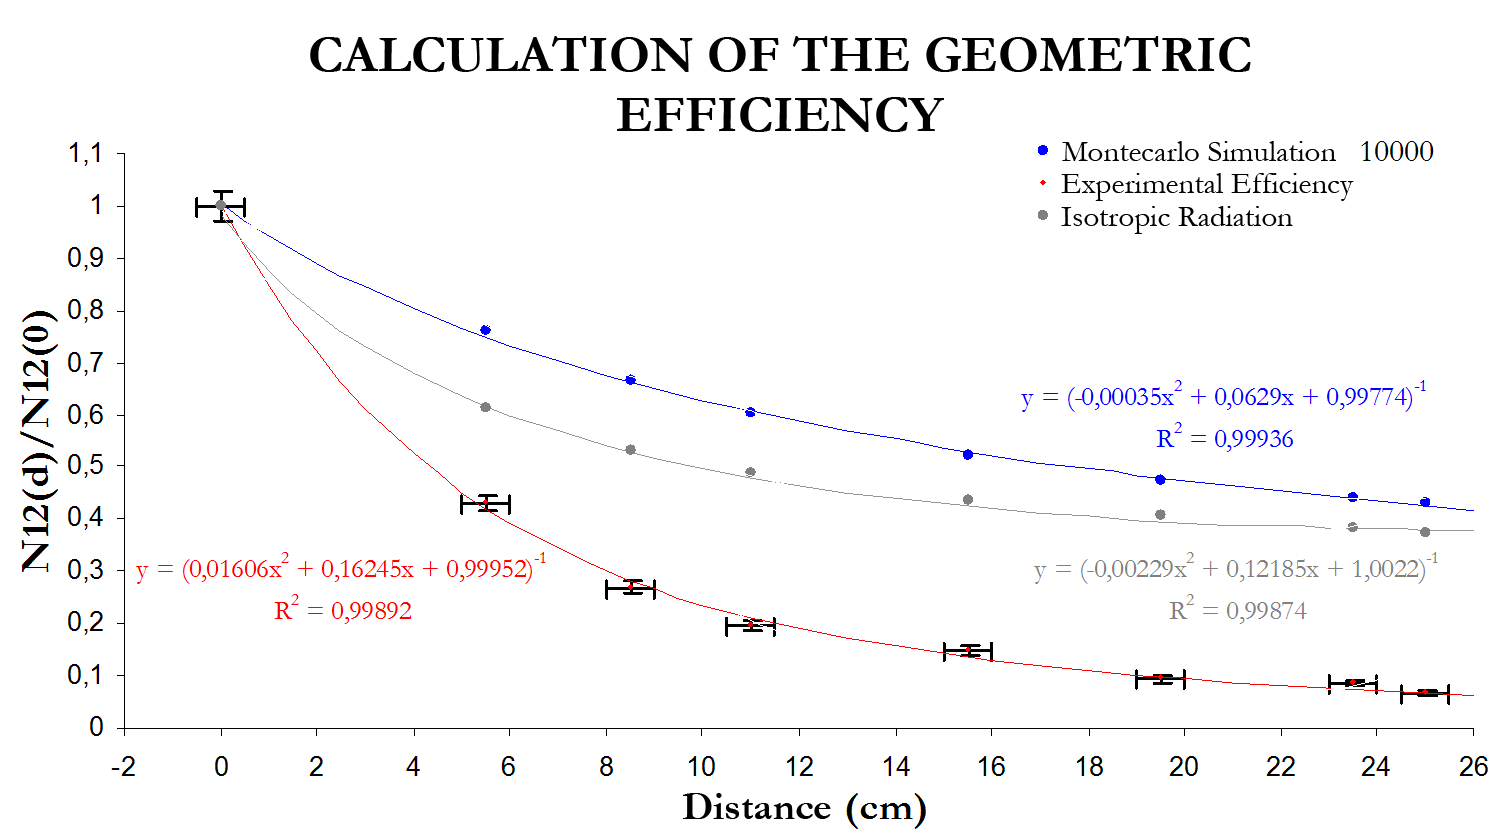
\includegraphics[width=\textwidth]{img/geoEff.png}\ec
				\caption[Comparison of experimental data with MC simulations]{Data for the MC simulation, the efficiency calculated experimentally with the error bars, and isotropic radiation. All curves are fit to curves whose dependency on the distance is proportional to the inverse square of the distance between scintillators.}\label{fig:geoeff}
			\efi

Despite the inconsistencies in values, both the curve simulation not isotropic and experimental follow a similar behavior, similar to a proportionality with $d^{-2}$.

Besides its slopes remain parallel above a large region from 6 cm more or less, where the experimental data has a lower error. This does not happen with to slope of the isotropic simulation, which is low but then comes back up.

So we can conclude that \textbf{the isotropic radiation is not a good model to represent the cosmic radiation}.

Assuming that the soft radiation has the same angular distribution as the hard one, can represent the relative fraction of hard and soft component as a function of the distance between scintillators. We can make a table of hard and soft components at different distances using the geometric efficiency calculated in this section, to be specific that obtained by MC simulation is more accurate and reliable.

Flux values for the hard and soft component obtained in the above at a distance of 30 cm section are taken into account, by correcting the geometric efficiency, and considering that, because two values were obtained for each obtained from settings for Lead and Aluminum, an average of the two will be used:

\bc
Average of the hard component at 30 cm: $J_h$ = 20 $\pm$ 2 m$^{-2}$s$^{-1}$\\
Average of the soft component at 30 cm: $J_s$ = 12 $\pm$ 4 m$^{-2}$s$^{-1}$\\
\ec
If these averages are corrected by dividing the geometric efficiency calculated by the MC for 30 cm, whose value turns out to be $\epsilon_{geo}$ = 0.3891, we obtain:

\bc
Hard component at 0 cm: $J_h$ = 51 $\pm$ 5 m$^{-2}$s$^{-1}$ = 62.2\% of the total flux\\
Soft component at 0 cm: $J_s$ = 31 $\pm$ 10 m$^{-2}$s$^{-1}$ = 37.8\% of the total flux\\
\ec

Doing the calculations, we obtain a data table like this one:


	\ctable [
	cap	    = {Comparison of the hard and soft flux for the MC and experimentf.},
 	caption = {Increasing values of d (error: $\pm$ 1 mm) with the relative fraction of hard and soft component in the case of the theoretical data and the experimental data. Calculation errors are not considered in these data.},
 	label   = {tab:MCflux},
 	pos	    = H,
	botcap
	]
	{c c c c c c c c c}
	{}
 	{\FL
		& &
		\multicolumn{3}{c}{\textbf{THEORY}} &
		\multicolumn{4}{c}{\textbf{EXPERIMENT}} \\
		\textbf{d (cm)} &
		\textbf{\pbox{.3\textwidth}{\pcen Geom.\\$\epsilon$\\[1ex]}} &
		\textbf{\pbox{.3\textwidth}{\pcen $J_h$\\[1ex](m$^{-2}$s$^{-1}$)\\[1ex]}} &
		\textbf{\pbox{.3\textwidth}{\pcen $J_s$\\[1ex](m$^{-2}$s$^{-1}$)\\[1ex]}} &
		\textbf{\pbox{.3\textwidth}{\pcen $J_d/J_s$\\[1ex]}} &
		\textbf{\pbox{.3\textwidth}{\pcen $J_h$\\[1ex](m$^{-2}$s$^{-1}$)\\[1ex]}} &
		\textbf{\pbox{.3\textwidth}{\pcen $J_s$\\[1ex](m$^{-2}$s$^{-1}$)\\[1ex]}} &
		\textbf{\pbox{.3\textwidth}{\pcen $J_d/J_s$\\[1ex]}} &
		\textbf{Error} \\
		\cmidrule(r){1-2}\cmidrule(rl){3-5}\cmidrule(l){6-9}
		0.0  & 1      & 150     & 30     & 5 & 51 & 31 & 2 & 1 \\
		5.5  & 0.7585 & 113.775 & 22.755 & 5 & 39 & 24 & 2 & 1 \\
		8.5  & 0.6647 & 99.705  & 19.941 & 5 & 34 & 21 & 2 & 1 \\
		11.0 & 0.6026 & 90.39   & 18.078 & 5 & 31 & 19 & 2 & 1 \\
		15.5 & 0.5236 & 78.54   & 15.708 & 5 & 27 & 16 & 2 & 1 \\
		19.5 & 0.4751 & 71.265  & 14.253 & 5 & 24 & 15 & 2 & 1 \\
		23.5 & 0.4398 & 65.97   & 13.194 & 5 & 22 & 14 & 2 & 1 \\
		25.0 & 0.4303 & 64.545  & 12.909 & 5 & 22 & 13 & 2 & 1
	\LL}


The ratio obtained between the hard and soft components is constant for both the tabulated data as to the experimental ones, so it follows that the angular distribution of both components is similar.

\section{Comparison of the experimental results for the flux with theory}

The table below shows a comparison between the calculated values and theory.

\begin{center}
\rowcolors{5}{lightgray}{lightgray}

	\ctable [
	cap	    = {Comparison of the hard and soft flux for the MC and experimentf.},
 	caption = {The values obtained experimentally and with the MC appear in color, a and b are the smaller and larger sides of the detectors, and d is a random separation between them.},
 	label   = {tab:thflux},
 	pos	    = H,
	botcap
	]
	{c c c c}
	{}
 	{\FL 
		\textbf{a (cm)} &
		\textbf{b (cm)} &
		\textbf{d (cm)} &
		\textbf{\pbox{.3\textwidth}{\pcen Fraction crossing both detectors (\%)\\[1ex]}} \\
		27 & 9 & 26 & 15 \\
		28 & 10 & 24 & 19 \\
		29 & 11 & 22 & 23 \\
		31 & 10 & 23.5 & 8.6 (EXP) \\
		31 & 10 & 23.5 & 43.9 (MC)
	\LL}
\end{center}

Now, since $J = J_0 \pi/2$, the total flux $J_0$  in the vertical direction, \textit{i.e.}, perpendicular to the detectors, can be calculated. From the value of the number of coincidences due to the hard and soft components obtained in the previous section, and the total flux, the following values are obtained together with their uncertainty:


	\ctable [
	cap	    = {Comparison of the flux values (theory and experiment).},
 	caption = {Theoretical values taken from \cite{prd:96} compared to those obtained experimentally.},
 	label   = {tab:thExp},
 	pos	    = H,
	botcap
	]
	{c c c c c c c}
	{}
 	{\FL
		&
		\multicolumn{3}{c}{\textbf{THEORY}} &
		\multicolumn{3}{c}{\textbf{EXPERIMENT}} \\
		\textbf{\pbox{.2\textwidth}{\pcen Flux\\(m$^{-2}$s$^{-1}$sr$^{-1}$)\\[1ex]}}&
		\textbf{Total} &
		\textbf{\pbox{.2\textwidth}{\pcen Hard\\$\sim\mu^+$\\[1ex]}} &
		\textbf{\pbox{.2\textwidth}{\pcen Soft\\$\sim e^+$\\[1ex]}} &
		\textbf{Total} &
		\textbf{\pbox{.2\textwidth}{\pcen Hard\\$\sim\mu^+$\\[1ex]}} &
		\textbf{\pbox{.2\textwidth}{\pcen Soft\\$\sim e^+$\\[1ex]}} \\
		\cmidrule(r){1-1}\cmidrule(rl){2-4}\cmidrule(l){5-7}
		\textbf{$J_0$}  &
		110 & 80 & 30 & 52 $\pm$ 9 & 32 $\pm$ 3 & 20 $\pm$ 6\\
		\textbf{$J$}  &
		180 & 130 & 50 & 82 $\pm$ 15 & 51 $\pm$ 5 & 31 $\pm$ 10
	\LL}

The obtained experimental data differ by 60\% from theory, due to the high voltage and that one of the scintillators is poorly attached to the light guide, which results in losses of photons that must reach the light guide. Furthermore, in the case of the soft component, we must take into account the absorption by the roof, which somewhat limits the amount of particles reaching the detectors.
